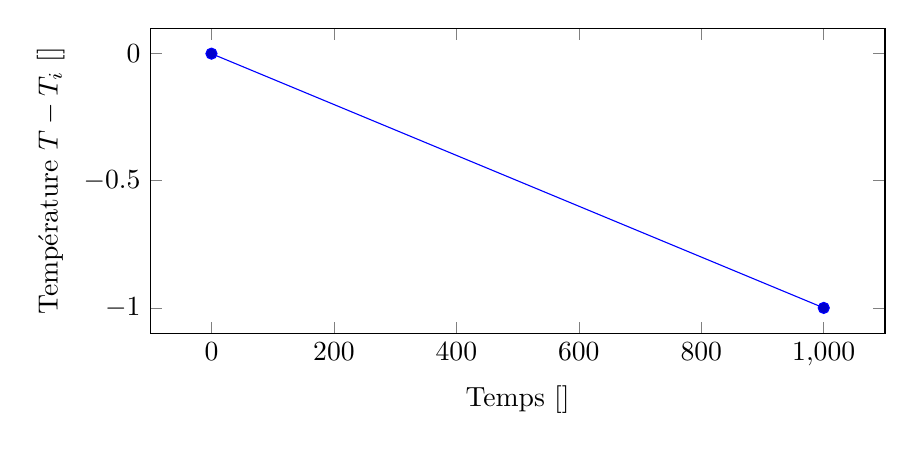
\begin{tikzpicture}
    \def\width{.9*\textwidth};
    \def\height{.5*\width};
    \def\spx{.25cm};
    \def\spy{1.25cm};
    \def\legx{.5cm};
    \def\legy{\legx};
    \def\prop{.45};
    
    \begin{axis}[name=TC,width={\width},height={\height},
    xlabel={Temps [\unit{\s}]},
    ylabel={Température $T - T_i$ [\unit{\degree}]},
%    xmin=0,xmax=75,ymin=0,ymax=.5/1000,
%    xtick={0,25,47,50,75,100},ytick={0,9.1120/100000,1.4452/10000,2.5/10000,5/10000,1/1000},
    legend style = {at={(.95,.95)},anchor = north east}
    ]
       \addplot coordinates {(0,0) (1000,-1)};
        
%        \legend{ \\};
    \end{axis}
\end{tikzpicture}